\documentclass[a4paper]{article}

\usepackage{graphicx}
\usepackage[utf8]{inputenc}

\hyphenation{ve-ri-fi-car FalaBrasil}

\title{Reconhecimento de Padrões em Erro no Reconhecimento
   Automático de Voz\\
   Mineração de Dados}

\author{Pedro Batista - pedro@ufpa.br}

\begin{document}

\maketitle

\section{Reconhecimento de Voz Baseado em HMM}\label{sec:rec}

Quando se fala em Reconhecimento Automático de Voz (RAV) a
principal abordagem encontrada na literatura é a probabilística,
especificamente Modelos Ocultos de Markov (HMM - Hidden Markov Model)\cite{htkbook,propor10}.
Existem também trabalhos que usam Inteligencia Artificial para
reconhecer o áudio, porém neste trabalho estamos usando HMM.

Em HMM, são criados modelos para cada fonema existente na lingua,
isto é, com um modelo para cada tipo de som podemos criar qualquer
palavra. Com esses modelos precisamos de um software chamado
decodificador, este recebe os modelos e o audio de entrada,
tendo isso, o decodificador é capaz de transcrever sua entrada.

\section{Erros de Reconhecimento}

É importante notar que o reconhecimento usando a técnica citada
na Seção~\ref{sec:rec} está sujeito a erro, e este trabalho, tem
como objetivo encontrar e corrigir um padrão de erro. Para entender
melhor abaixo descrevemos uma possível saída de um decodificador.

Um decodificador pode nos dar como saída o score de cada frame no
processo de reconhecimento, isto é, um grafo (aqui chamado lattice) onde seus links
representam uma transição entre palavras. A transição tem um determinado
peso (score) que o decodificador gera, comparando os modelos com a entrada.
O objetivo é chegar no final deste grafo com o
menor score possível, guardando as palavras (nós) pelo qual passou,
gerando assim a sentença reconhecida. Para ilustrar é mostrado abaixo
uma lattice.

\begin{verbatim}
VERSION=1.0
UTTERANCE=/projetos/datalaps/voz/tidigits16kwav/test/testboymn82a.mfc
lmname=network
lmscale=1.00   wdpenalty=0.00  
acscale=1.00  
vocab=dicionario.dic
N=75   L=185  
I=0    t=0.00  W=!NULL               
I=1    t=0.02  W=SENT-START          v=1  
I=2    t=0.03  W=SENT-START          v=1  
I=3    t=0.05  W=oh                  v=1  
I=4    t=0.05  W=SENT-START          v=1  
I=5    t=0.06  W=oh                  v=1  
I=6    t=0.08  W=eight               v=1  
.
.
.
I=73   t=1.14  W=!NULL               
I=74   t=1.14  W=SENT-END            v=1  
J=0     S=0    E=1    a=-103.10   l=0.000   d=:sil[2],0.01,-43.42:sil[4],0.01,-59.69:
J=1     S=0    E=2    a=-151.93   l=0.000   d=:sil[2],0.01,-40.87:sil[2],0.01,-55.74:
sil[4],0.01,-55.32:
J=2     S=1    E=3    a=-355.51   l=0.000   d=:ow1[2],0.01,-75.01:ow1[3],0.01,-188.56:
ow1[4],0.01,-91.94:
J=3     S=0    E=4    a=-267.09   l=0.000   d=:sil[2],0.01,-40.87:sil[2],0.01,-53.19:
sil[2],0.01,-49.71:sil[4],0.01,-63.11:sil[4],0.01,-60.21:
.
.
.
J=184   S=72   E=74   a=-1045.06  l=0.000   d=:sil[2],0.01,-57.30:sil[2],0.01,-62.06:
sil[2],0.01,-55.21:sil[2],0.01,-57.45:sil[2],0.01,-53.44:sil[2],0.01,-56.24:
sil[2],0.01,-59.72:sil[4],0.01,-58.34:sil[4],0.01,-57.14:sil[4],0.01,-59.52:
sil[4],0.01,-59.28:sil[4],0.01,-54.67:sil[4],0.01,-55.36:sil[4],0.01,-53.63:
sil[4],0.01,-62.21:sil[4],0.01,-58.88:sil[4],0.01,-66.78:sil[4],0.01,-57.83:
\end{verbatim}

As linhas iniciadas com \texttt{I} ilustram os estados, e a estes estão vinculados
palavras (\texttt{W}), as transições entre elas, são as linhas iniciadas com \texttt{J}. A
transição \texttt{J}, é de \texttt{S} para \texttt{E}, e tem o peso \texttt{a} (acústico),
e \texttt{l} (linguístico), o peso \texttt{a} é detalhado em \texttt{d}, sendo que \texttt{d}
nos fornece os dados da seguinte forma: \texttt{:n,t,s:}, onde \texttt{n} representa
o estado da HMM, \texttt{t} o tempo de permanência nesse estado e \texttt{s} o score
obtido nesse estado e tempo. Uma descrição mais detalhada deste tipo de lattice pode 
ser encontrada em~\cite{htkbook}.

\section{Metodologia}

Tendo acesso a lattice e a sentença que deveria ter sido reconhecida (correta) de um
determinado som podemos determinar se houve um erro ou não. Um erro
frequentemente significa que a sentença com maior score (reconhecida) não foi a correta.
Porém, a correta está quase sempre no rank das 5 melhores.

Uma vez que determinada as sentenças reconhecida e a correta podemos verificar, que
elas compartilham muitas transições, e comumente o erro acontece em alguns poucos
frames, onde certo fonemas se confundem (ponto de confusão). Na Fig~\ref{fig:score} é mostrado
um gráfico do score pelos frames de duas sentenças, a reconhecida e a correta de um processo
de reconhecimento.

\begin{figure}[!h]
  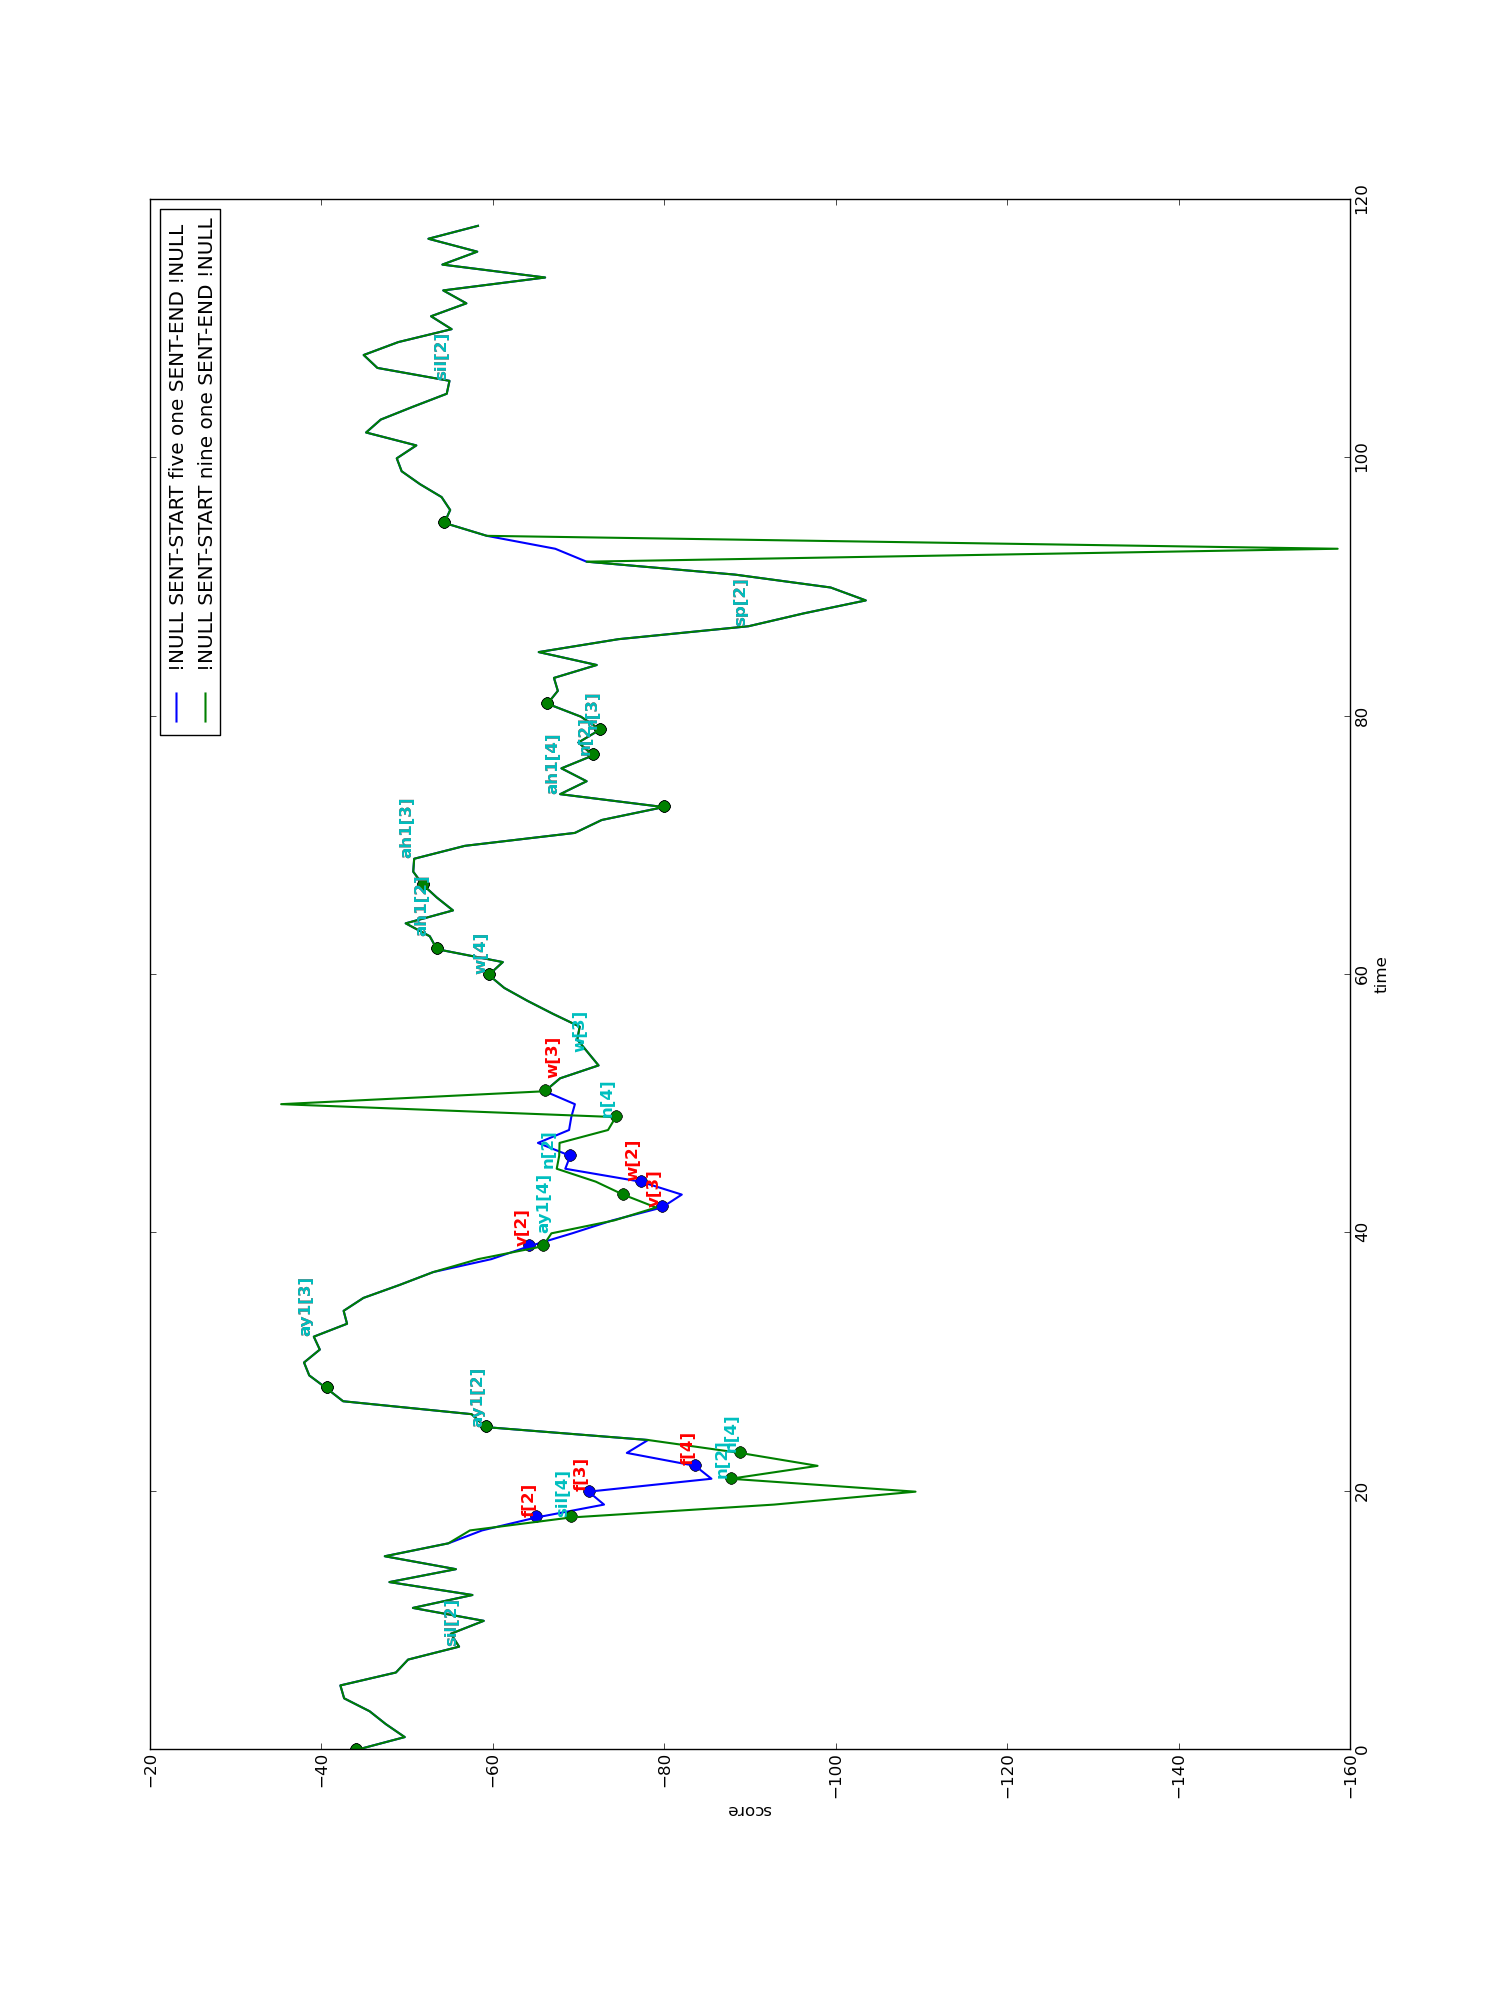
\includegraphics[height=20cm]{out}
  \caption{Score de reconhecimento de duas sentenças, em verde a correta e em azul a reconhecida.}
  \label{fig:score}
\end{figure}

Podemos observar, que próximo do frame 20, houve uma confusão principalmente entre os fonemas 
\textbf{f} e \textbf{n}, neste caso o \textbf{n} que pertence a sentença correta,
ficou com score menor que o \textbf{f} (reconhecida), ocasionando o erro do reconhecimento. Algo parecido
acontece próximo do frame 40.

Acredita-se que observando parâmetros do áudio seja possível, encontrar um padrão de confusão e 
corrigi-lo, para isso serão usadas técnicas de mineração de dados.

\section{Colaboração}

É importante notar que este trabalho está sendo desenvolvido, pelo grupo FalaBrasil, do
Laboratório de Processamento de Sinais, e que Pedro Batista, é apenas um membro do grupo de
desenvolvimento.

\bibliographystyle{plain}
\bibliography{bib.bib} 
\end{document}
